\section{Methodology}
\subsection{Overview}
This project consists of three main units: a discharge flow control unit, a discharge collection  unit, and a main control unit. 
\subsection{Discharge flow control unit}
This unit will be used for controlling the flow at the end of the pipe system. It will utilize a ball valve installed on the existing machine. It is required that the valve aperture is controlled in steps specified by the user. However, the ball valve will be controlled by a driver based on a micro-controller. Some of the actuation mechanisms that can be applied for this purpose include :

\subsubsection{Stepper linear actuator}

A stepper motor converts a full rotation to small equal steps. The step size vary from one motor to the other.It will be used in this case to drive the handle of the ball valve. A mechanical interface such as a level system will be used between the motor and handle.

\subsubsection{Piezoelectric Actuator}

A Piezoelectric actuator converts electrical energy to mechanical displacement. It can provide high precision displacements with a large output force. It will be mounted between the handle lever and a stationary surface. When energised, the actuator will displace the lever and hence turning the valve. It is responsive to small variation in voltage.

\par

The choice between these mechanisms will depend on the following factors :
\begin{enumerate}
    \item Torque requirements  of the ball valve. 
    \par The piezoelectric actuator is suited for higher torque requirements as compared to the stepper motor. 
    \item Step sizes
    \par Stepper motors are restricted to step sizes above their step angle which is typically 0.9 $^{\circ}$. Piezoelectric actuators have a positioning accuracy of 0.3 mm.
\end{enumerate}

\subsection{Discharge collection unit}
This unit will form the core part in the automation of the discharge collection. It will consists of the following : a flow diversion sub-unit, a discharge collection tank, an outlet valve, weight and temperature measurement sub-units. 
 
\subsubsection{Flow diversion sub-unit}
This unit will be responsible for diverting the flow of the discharge from the main pipe system to the discharge collection tank. It will be required to have a fast response time of about a few milliseconds. It is also expected to divert the flow with minimum splashes and leakages into the discharge collection tank. This unit will consist of a flap, and an actuation unit. The design of the flap will be based on the following factors :
\begin{enumerate}
    \item Size \newline
    The size of the flap should be considered such that it will be able to fully cover the inlet of the discharge collection pipe. 
    \item Shape \newline
    The shape of the flap should be such that it can divert the discharge away from the discharge collection unit with minimum spillage into the collection pipe. A funnel-shaped flap will be considered for this case.
    \item Material \newline
    The flap will always be in contact with the discharge fluid. This necessitates the flap to be a resistant to rust. The flap will also be actuated by a driver, and in order to achieve a fast response, the material of flap should be light.
\end{enumerate}
\par
The following mechanisms will be considered for the actuation of the flap :
\begin{enumerate}
    \item Electromagnets \newline
    This mechanism generates a magnetic effect on application of voltage. This will attract the metallic flap and hence opening the discharge collection pipe. The flap will be returned by a spring system in order to close the pipe.
    \item Motors \newline
    This mechanism will operate by driving the lid back and forth through an interface. The interface between the lid and the motor can be either a screw or a nut and a bolt. As the motor rotates, it either screws in or out the screw or the bolt and hence opening or closing the pipe.
\end{enumerate}
\par
The choice between this two type of methods will depend on the following factors :
\begin{enumerate}
    \item Force requirements \newline
    This refers to the force required to maintain the flap and hence the pipe open or closed. This will be affected by the stream of the discharge landing on the flap. Electromagnets can be adapted to produce more force by increasing the supply voltage. However, the motor will have to be replaced by another motor with more torque.
    \item Voltage requirements \newline
    Electromagnets tend to require higher voltages to produce the same force as a motor.
\end{enumerate}
\subsubsection{Discharge collection tank}
This unit will be used to collect the discharge temporarily at each step during the experiment. The weight and temperature of the discharge will be measured within the tank. The design of the tank will involve the consideration of the following factors :
\begin{enumerate}
    \item Position \newline
    The position of the tank will influence size of the collection pipe and also the positioning of the outlet valve. The tank will be required the elevated above the reservoir in order to eliminate the need for a pump for pump out the discharge. 
    \item Insulation \newline
    Since the temperature of the discharge is taken in this tank, the influence of the external environment will have a negative impact on the readings. The tank is therefore required to maintain internal environment with minimal effect from the external environment. 
    \item Shape \newline 
     The shape of the tank will determine will influence weight measurement, and the positioning of the outlet valve.
\end{enumerate}
\subsubsection{Outlet valve}
This valve will be responsible to emptying the discharge collection tank into the reservoir. The design of this valve will be based on the following factors :
\begin{enumerate}
    \item Position \newline 
    The position of the outlet valve will be critical since it determines how fast the mini collection tank drains into the reservoir.
    \item Size. \newline
    The size of the valve will also determine how fast the tank empty to the reservoir. 
\end{enumerate}
\subsubsection{Weight measurement sub-unit}
This sub-unit will be used to measure the weight of the discharge in the collection tank. The following approaches will be considered for this unit :

\begin{enumerate}
    \item Ultrasonic \newline
    Ultrasonic waves will be used to determine the depth of the discharge in the tank. This will be used with the cross-sectional area of the tank, and the density of the tank to determine the weight of the discharge based on following equation.
    \item Load cells \newline
    This will utilize load cells distributed below the discharge collection tank. The average of the output of the load cells will be averaged. 
\end{enumerate}

\par
The choice between these two approaches will depend on the following factors :
\begin{enumerate}
    \item Resolution. \newline
    The refers to the smallest unit that can be measured by the measurement device. The resolution of ultrasonic waves will depend on the pulse rate of the ultrasonic wave generator. 
    \item Reliability. \newline
    The application of ultrasonic waves requires the consideration of other factors such as the cross-sectional area and the shape of the tank. This will not be the case with the load cells. This makes the measurements using the load cells more reliable than those utilizing ultrasonic waves.
\end{enumerate}

\subsubsection{Temperature measurement sub-unit}
This sub-unit will be required to measure the temperature of discharge in the tank. The following types of temperature measurement methods will be considered in the choice of a suitable sub-unit:
\begin{enumerate}
    \item Contact temperature measurement \newline
    The measuring device will be placed inside the tank and thus it will come into contact into contact with the discharge.
    \item Contactless temperature measurement \newline
    In the non contact type, the measuring device  will not come into contact with the discharge.
\end{enumerate}
\par
The choice between the two technologies will be based on the following :
\begin{enumerate}
    \item Sensitivity \newline 
     This refers to how responsive the device is to the smallest change in the environment. A contact temperature measurement unit is predicted to have a higher sensitivity as compared to a contactless unit.
     \item Reliability \newline
     The application of a contactless temperature unit will require the consideration of the stimuli between the unit and the environment being probed. This is not the case with a contact temperature measurement unit as there is a direct interface with the environment being probed.
\end{enumerate}

\subsection{Interface and Control}
 This unit will take user input through an interface, and process the input with the data from the system using an application logic running in a micro-controller. The application logic will be as shown in figure \ref{fig:control_flow}. The results of the process will be displayed on the interface. 
\begin{figure}
    \centering
    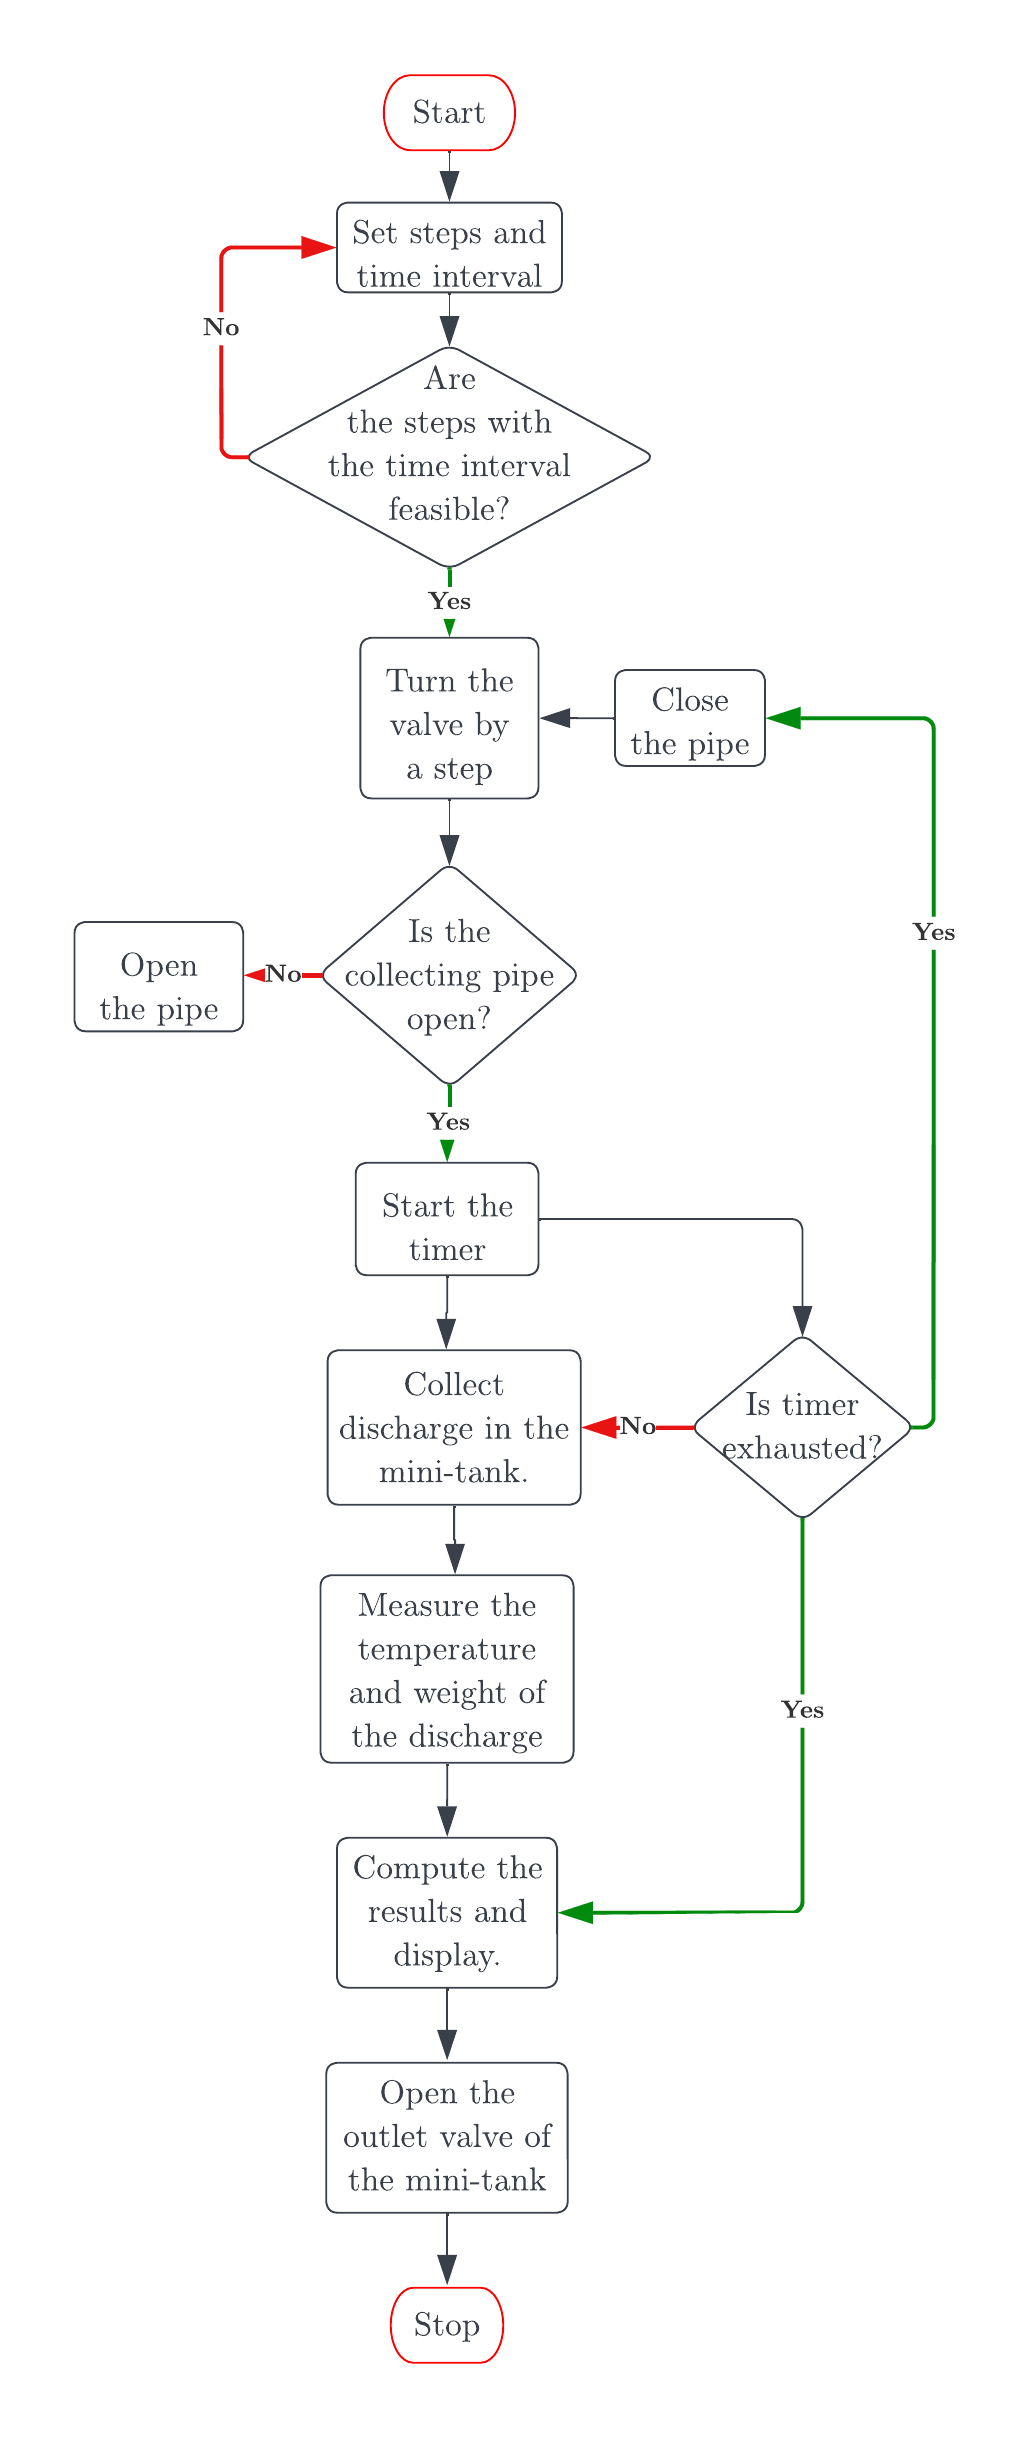
\includegraphics[width=\textwidth,height=\textheight,keepaspectratio]{Figures/Control_flow.png}
    \caption{Application logic}
    \label{fig:control_flow}
\end{figure}
\subsubsection{Processing sub-unit}
This sub-unit executes the application logic, send instructions to the actuators, and reads inputs from sensors in the system. A micro-controller or a fully developed computer board such as Raspberry Pi may be considered for this application. The choice of a micro-controller or a computer chip will be determined by the following factors. 
\begin{enumerate}
    \item \ac{GPIO}s \newline
    These form the primary interface between a micro-controller and the external circuitry. They can be used for several purposes such as analog signal I/O, counter/timer, digital signal I/O, and serial communication. A group of these pins forms a port. The number of pins and hence the size of the port are two important factors that are to be considered in the choice of a micro-controller. 
    \par
    Some devices such as LCD displays with touch capability require bigger ports as many devices require many GPIOs to control them. 
    \item Processing Power  \newline
    This refers to the processing capacity of a micro-controller. A multi-core processor is faster and consumes more power as compared to a single-core processor. A multi-core processor can also render intense graphics on displays. The amount of input processing will guide one in choosing the best micro-controller or microprocessor for the task.
\end{enumerate}
\subsubsection{Interface}
This will provide for a human machine interaction. It will allow one to enter the required experiment parameters like start and stop or reset of the experiment, and read the processed results which will include parameters such as the weight and temperature of the discharge. Some of the interfaces that will be considered in this project are:
\begin{enumerate}
    \item \textbf{LCD with Keypad} \newline
    One can navigate, read and provide input where it is required on the LCD display using the keypad. 
    \item \textbf{LCD with touch capability} \newline
    One can navigate the interface easily by touching and using a virtual keyboard to provide input.
    \item \textbf{LCD with Knobs} \newline
    The interface will be entirely controlled by knobs, navigation from page to page, and parameter input.
\end{enumerate}

The choice of one of the three means to interface with the machine will entirely depend on the following factors.

\begin{enumerate}
    \item Aesthetics \newline
    This refers to the perception of the user while operating the interface. A touch screen is minimalistic, and its aesthetics can be improved easily by adding relatively beautiful graphics in the software. This might not be the case with the case of LCD with knobs. Any attempts to improve its aesthetics might require the addition of knobs. This might clutter the interface.
    \item Ergonomics \newline
    This refers to the impact of the interface on the user, and the ease of operation. LCD display with a keypad interface can be operated even in a moist environment. This might not be the case with an LCD display with touch capability.    
    \item Size  \newline
    This refers to the size of the display with regard to the size of the contents to be displayed. Fewer contents can fit any of the mentioned displays but the operability of the contents in the display should be considered. 
\end{enumerate}